\documentclass{article}
\usepackage{amsmath}

\DeclareMathOperator*{\argmax}{arg\,max}
\DeclareMathOperator*{\argmin}{arg\,min}

\usepackage{amsfonts}

\usepackage{tikz}
\usetikzlibrary{fit,positioning,shapes}

\usepackage[shortlabels]{enumitem}

\usepackage{algorithm}
\usepackage{amssymb}
\usepackage{booktabs}
\usepackage{algpseudocode}

\textwidth=7.6in
\textheight=9.9in
\topmargin=-.9in
\headheight=0in
\headsep=.5in
\hoffset=-1.5in
\setlength\parindent{0pt}


\begin{document}

\begin{center}
    \Large{\textbf{Problem Set 3 Solutions}} \\[0.25ex]
    Calvin Walker
\end{center}
\textbf{1.}
\begin{enumerate}[(a)]
    \item Consider the M-projection with the factored approximation $Q(X, Y) = Q(X)Q(Y)$, \begin{align*}
        D(P || Q) &= \sum_{X, Y} P(X, Y) \log \frac{P(X, Y)}{Q(X)Q(Y)} \\[0.5ex]
        &= \mathbb{E}_P[\log P(X, Y) - \log Q(X)Q(Y)] \\[0.5ex]
        &= \mathbb{E}_P[\log P(X, Y)] - \bigg(\mathbb{E}_p[\log Q(X)] + \mathbb{E}_p[\log Q(Y)]\bigg) \pm \log(P(X)P(Y)) \\[0.5ex]
        &= \mathbb{E}_p \bigg[\log \frac{P(X, Y)}{P(X)P(Y)}\bigg] + \mathbb{E}_p \bigg[\log \frac{P(X)}{Q(X)}\bigg] + \mathbb{E}_p \bigg[\log \frac{P(Y)}{Q(Y)}\bigg]
    \end{align*}
    Letting $Q^*_M = P(X)P(Y)$, \begin{align*}
        D(P || Q) &= D(P || Q^*_M) + \mathbb{E}_p \bigg[\log \frac{P(X)}{Q(X)}\bigg] + \mathbb{E}_p \bigg[\log \frac{P(Y)}{Q(Y)}\bigg]
    \end{align*}
    Thus, $D(P || Q) \geq D(P || Q^*_M)$, and $Q^*_M = P(X)P(Y)$ minimizes the M-projection. 
    \item \begin{align*}
        \theta^* &= \argmax_\theta \prod_{i = 1}^{M}Q(X^{(i)} ; \theta) \\[0.5ex]
        &= \argmin_\theta \sum_{i = 1}^{M} - \log Q(X^{(i)} ; \theta) \\[0.5ex]
        &= \argmin_\theta \sum_{i = 1}^{M} - \log Q(X^{(i)} ; \theta) + P(X^{(i)})
    \end{align*}
    So if the sample size $M$ is significantly large, \begin{align*}
        \theta^* &=  \argmin_\theta \ \mathbb{E}_P \bigg[\log \frac{P(X)}{Q(X ; \theta)} \bigg] \\[0.75ex]
        &= \argmin_\theta \ D(P || Q(X ; \theta))
    \end{align*}
    Therefore, the MLE solution $\theta^*$ minimizes the KL-Divergence $D(P || Q(X ; \theta))$, and is equivalent to solving for the M-projection $D(P||Q)$. 
\end{enumerate}
\textbf{2.} 
\begin{enumerate}[(a)]
    \item 
    \item \textcolor{white}{{x}}
    \begin{figure}[th]
        \centering
        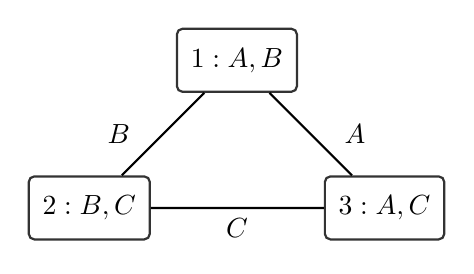
\begin{tikzpicture}[xscale=1.25,yscale=1.25]
            \tikzstyle{latent}=[rectangle, rounded corners=2pt, minimum size = 8mm, inner sep=5pt, thick, draw = black!80, node distance = 10mm]
            \tikzstyle{observed}=[rectangle, minimum size = 7mm, inner sep=0pt, thick, draw = black!80, node distance = 10mm,fill=gray!50]
            \tikzstyle{connect}=[thick]
            {\node[latent] (12) at (0,0.75){$1: A, B$};
            \node[latent] (23) at (-1.5,-0.75){$2: B, C$};
            \node[latent] (13) at (1.5,-0.75){$3: A, C$};
\node (x2) at (-1.2,0){$B$};
            \node (x3) at (0,-0.95){$C$};
            \node (x1) at (1.2,0){$A$};}
\path (12) edge [connect] (23);
            \path (23) edge [connect] (13);
            \path (13) edge [connect] (12);
        \end{tikzpicture}
        \caption{Example Cluster Graph}
        \label{fig:bethe-cluster-graph}
    \end{figure}

    Consider the above Cluster Graph for a pairwise MRF over three binary variables $A$, $B$, and $C$. We can satisfy the local consistency constraints with the following clique beliefs: 
\begin{gather*}
            \beta_{1}(A, B) =
            \begin{bmatrix}
                0.3 & 0.2\\ 0.2 & 0.2
            \end{bmatrix} \;
\beta_{2}(B, C) =
            \begin{bmatrix}
                0.3 & 0.2\\ 0.2 & 0.3
            \end{bmatrix}\;
\beta_{3}(A, C) =
            \begin{bmatrix}
                0.2 & 0.3 \\ 0.3 & 0.2
            \end{bmatrix}
    \end{gather*}
    Such that the sepset marginals are given by: $\mu_{1,3}(A) = \mu_{1,2}(B) = \mu_{2,3}(C) = (0.5, 0.5)$. However, if we sum over the possible outcomes: \begin{align*}
        \sum_{A, B, C} P(A, B, C) = 6 \bigg(\frac{18}{125}\bigg) + 2 \bigg(\frac{8}{125}\bigg) = \frac{124}{125} \neq 1
    \end{align*}
    So the parameterization does not correspond to a valid probability distribution, and we can see for a cluster graph that is not a tree, the marginal polytope is strictly contained by the local consistency polytope. 
\end{enumerate}


\textbf{3.} \begin{enumerate}[(a)]
    \item 
\end{enumerate}

\end{document}